%\lipsum[1-20]

Chapter~\ref{chp:bgm} has provided a framework for modeling the self-assembly of a polyhedron using a Markov process. When using a transition rate matrix of the form 
\begin{align}
  \label{eq:Qdef_rep}
  Q_{jk} =
  \begin{cases}
   S_{jk}e^{-\beta\left(E_{jk} - E_{j}\right)} & \text{if } [x^j] \leftrightarrow [x^k]  \\
   -z_j       & \text{if } j = k \\
   0 & \text{else}
  \end{cases}
\end{align}
the intermediate energies $E_j$ and transition barrier energies $E_{jk}$ must be specified. Using minus the number of closed edges in an intermediate has a nice, physically motivated interpretation. The choice of barrier heights, however, has not yet been addressed. Using information of an intermediate's geometric configuration space that can be gathered using our manifold reflected Brownian motion scheme, we derive energy barrier heights and thus the rate matrix $Q$. This combination of combinatorial and geometric structure provides a unique insight into the various themes of self-assembly.

\section{Deriving Rates}

Consider the process of adding a face to an intermediate. In the combinatorial configurations space this is a transition from one node of the graph to another. However, for this transition to occur in a more physical setting, the geometry of the intermediate plays a large role. One can imagine that there are geometric configurations are contorted in a way as to prevent a face from being added at a particular location. For instance consider the linkage of two triangles as an intermediate of the tetrahedron. Since the combinatorial configuration space is rather trivial, adding a face will results in the rigid linkage of three triangles all sharing a vertex. Since the equilateral triangle has angles of $\frac{\pi}{3}$, the angle between the two edges of the two triangle linkage that the third face attaches to must be close to $\frac{\pi}{3}$ for it to attach easily. We extend and formalize this idea for face attachment on a Building Game intermediate to obtain the rates we desire.

%Since we assume that each polyhedron is composed solely of triangles, each attachable face will have three vertices. For each of these vertices, there is either $0, 1,$ or $2$ vertices on the existing intermediate that they will attach to. If there are zero vertices on the intermediate that the vertex on the new face combines with, it means that the attachment occurs 


If there are three vertices $v_a, v_b, v_c$ in the intermediate that each combine with one of the three vertices on the added triangle, and $(v_a, v_b)$ and $(v_b, v_c)$ are edges in one of the intermediate's existing triangles, the rate of attachment for the face is given by the proportion of time the configuration--undergoing manifold reflected Brownian motion--has $\frac{\pi}{3} - \epsilon < \angle( v_a, v_b, v_c) < \frac{\pi}{3} + \epsilon$. Here $\epsilon$ is a parameter reflecting how close to the ideal angle the configuration must be in order to allow attachment. If there are no such triplets $v_a, v_b, v_c$ where a face is being attached, the attachment occurs at a unit rate. If there are more than one triplet $v_a, v_b, v_c$, the attachment rate is averaged across each such triplet. Taking this empirical rate and summing over the other faces corresponding to the degeneracies of the transition of interest, the empirical forward transitions rates $\hat{Q}_{jk}$ are derived. By comparing these computed rates with the analytic form for our transition rate matrix, we can derive the barrier heights $E_{jk}$ for each transitions. Since the barriers are symmetric, this information also gives the reverse transition rates $Q_{kj}$.
\begin{align}
\hat{Q}_{jk} &= Q^0_{jk} \\
	&= S_{jk}e^{\beta_0(E_{jk} - E_j)} \\
E_{jk} &= E_j-\frac{1}{\beta_0}\log\left(\hat{Q}_{jk}/S_{jk}\right)
\end{align}
Here $\beta_0$ is the inverse temperature used to derive the barriers from the empirical computations. Since 
\begin{align}
Q_{jk} 	&= S_{jk}e^{\beta(E_{jk} - E_j)} \\
 &= S_{jk} e^{-\beta\left(E_j-\frac{1}{\beta_0}\log\left(\hat{Q}_{jk}/S_{jk}\right) - E_j\right)} \\
 &= S_{jk}\left(\hat{Q}_{jk}/S_{jk}\right)^{\frac{\beta}{\beta_0}},
\end{align}
the choice of $\beta_0$ effectively specifies the units of $\beta$. Typically, we choose $\beta_0 = 1$.

To derive the empirical rates, each intermediate was simulated for $10,000,000$ steps with a stepsize of $h = 0.05$. By storing each of the relevant angles either step by step, or in a histogram, the rates can be computed for each choice of $\epsilon$ at a later time as needed.

\section{Self-Assembly Statistics}

After we have computed the rate matrix $Q$ for the octahedron as a function of $\epsilon$ and $\beta$, we are now able to compute the different statistics derived in section~\ref{sec:StochMod}. 
\begin{figure}[ht]
\centering
  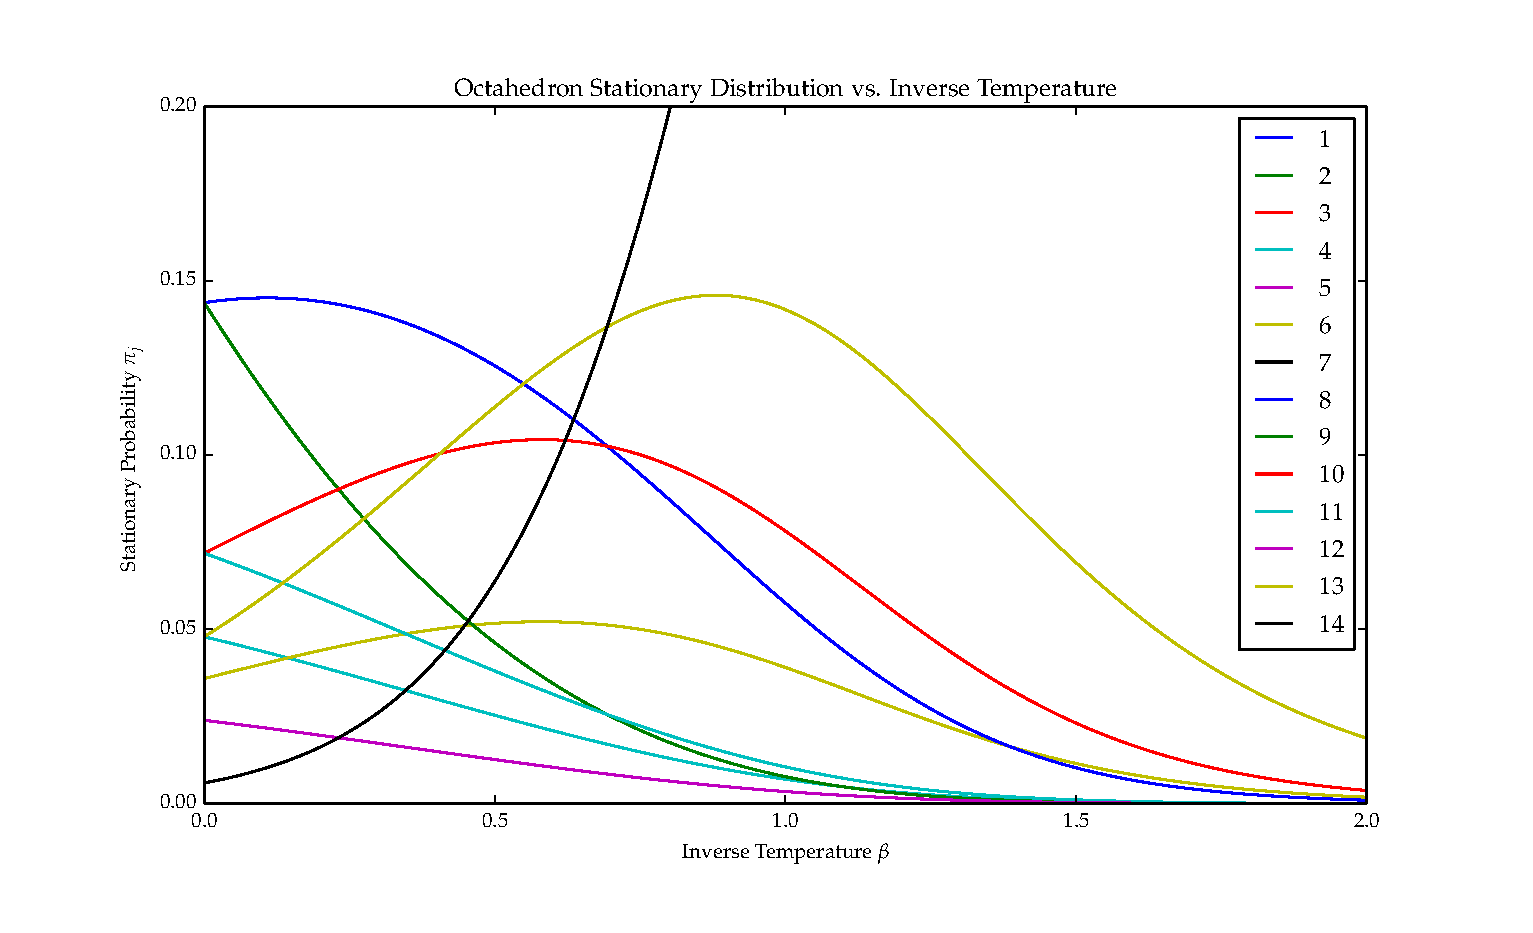
\includegraphics[scale=0.6]{images/octahedron_pi.eps}
\caption{Octahedron stationary distributions as a function of $\beta$.}
\label{fig:OctaPi}
\end{figure}
For instance, the stationary distribution of each octahedron intermediate is plotted as a function of $\beta$ in figure~\ref{fig:OctaPi}.
\begin{figure}[ht]
\centering
  \includegraphics[scale=0.6]{images/octahedron_log_pi.eps}
\caption{Natural log of the octahedron stationary distributions as a function of $\beta$.}
\label{fig:OctaLogPi}
\end{figure}
To better view how these probabilities decay as the temperature decreases, figure~\ref{fig:OctaLogPi} presents the natural logarithm of these stationary probabilities.

With the rate matrix, we can also look at how the occupation probabilities change over time. 
\begin{figure}[ht]
\centering
  \includegraphics[scale=0.6]{images/octahedron_finite_dist.eps}
\caption{Occupation probabilities for Octahedron intermediates as a function of time.}
\label{fig:OctaFinDist}
\end{figure}
If the process begins with a single face, the probabilities diffuse through the graph according to $e^{Qt}e_1$ and eventually converge of the stationary distribution $\pi$ as $t \to \infty$. Figure~\ref{fig:OctaFinDist} shows how these occupation probabilities change over time.

Another way to visualize the dynamic behaviors of our Markov process is to look at individual transitions and the rates with which they occur.
\begin{figure}[ht]
\centering
  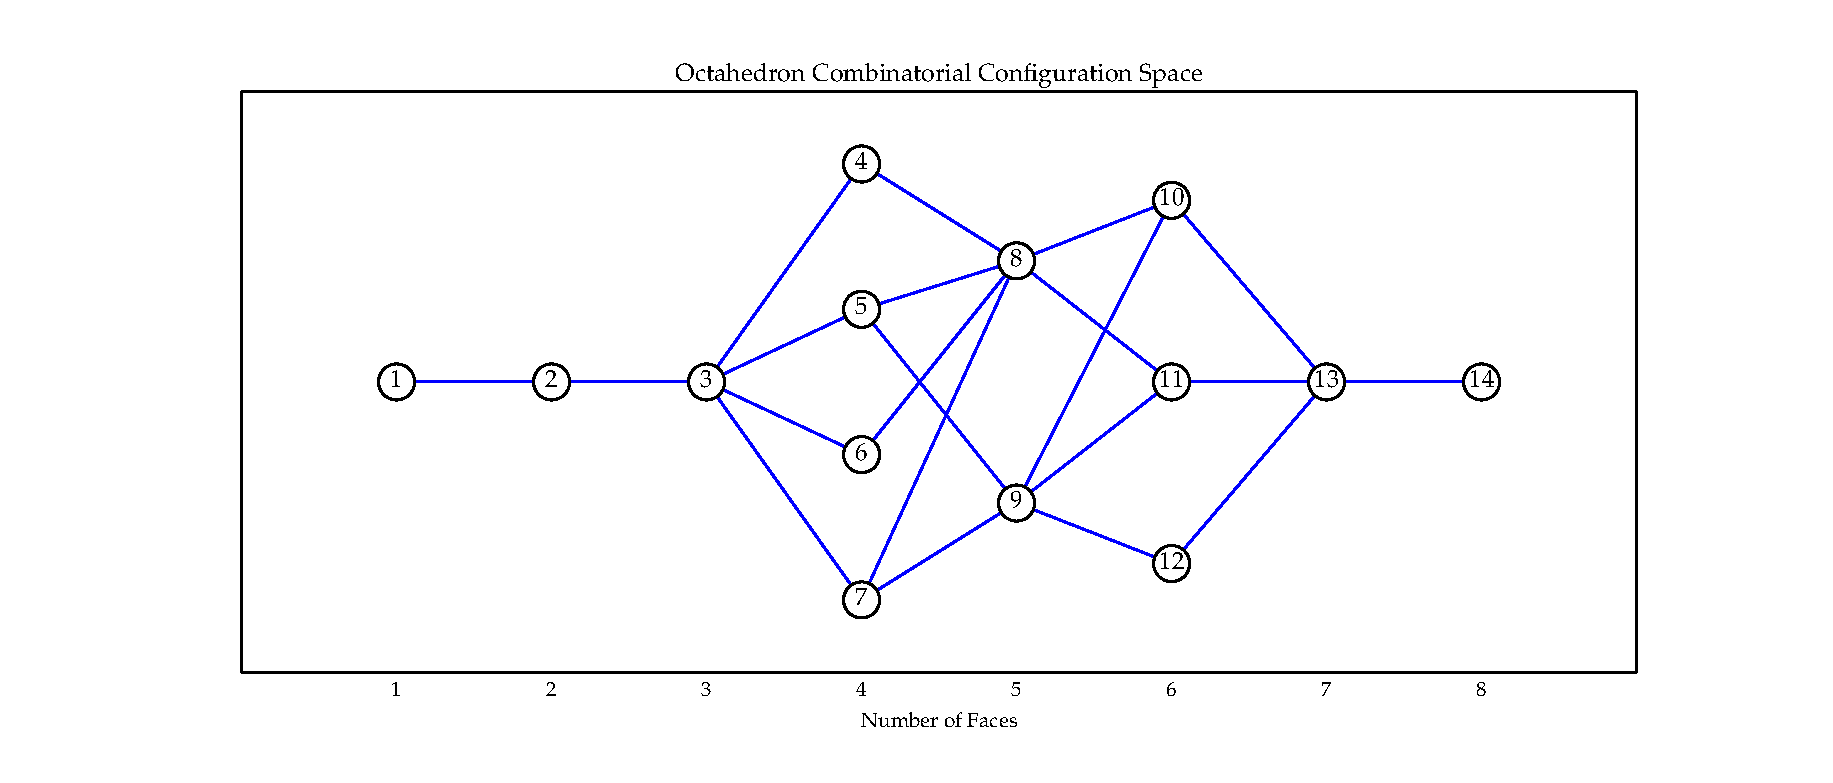
\includegraphics[scale=0.5]{images/octahedron_ccs.eps}
\caption{Combinatorial Configuration space for the Octahedron.}
\label{fig:OctaCCS}
\end{figure}
Figure~\ref{fig:OctaCCS} shows the octahedron combinatorial configuration space with the edges labeled with the joint transition rate $\pi_j Q_{jk} = \pi_k Q_{kj}$ for the choices $\beta = 0.8$ and $\epsilon = 0.5$.

Since our model uses the two parameters $\epsilon$ and $\beta$, it is of particular interest to examine how the choice of these parameters affects the behaviors of the Markov process. 
\begin{figure}[ht]
\centering
  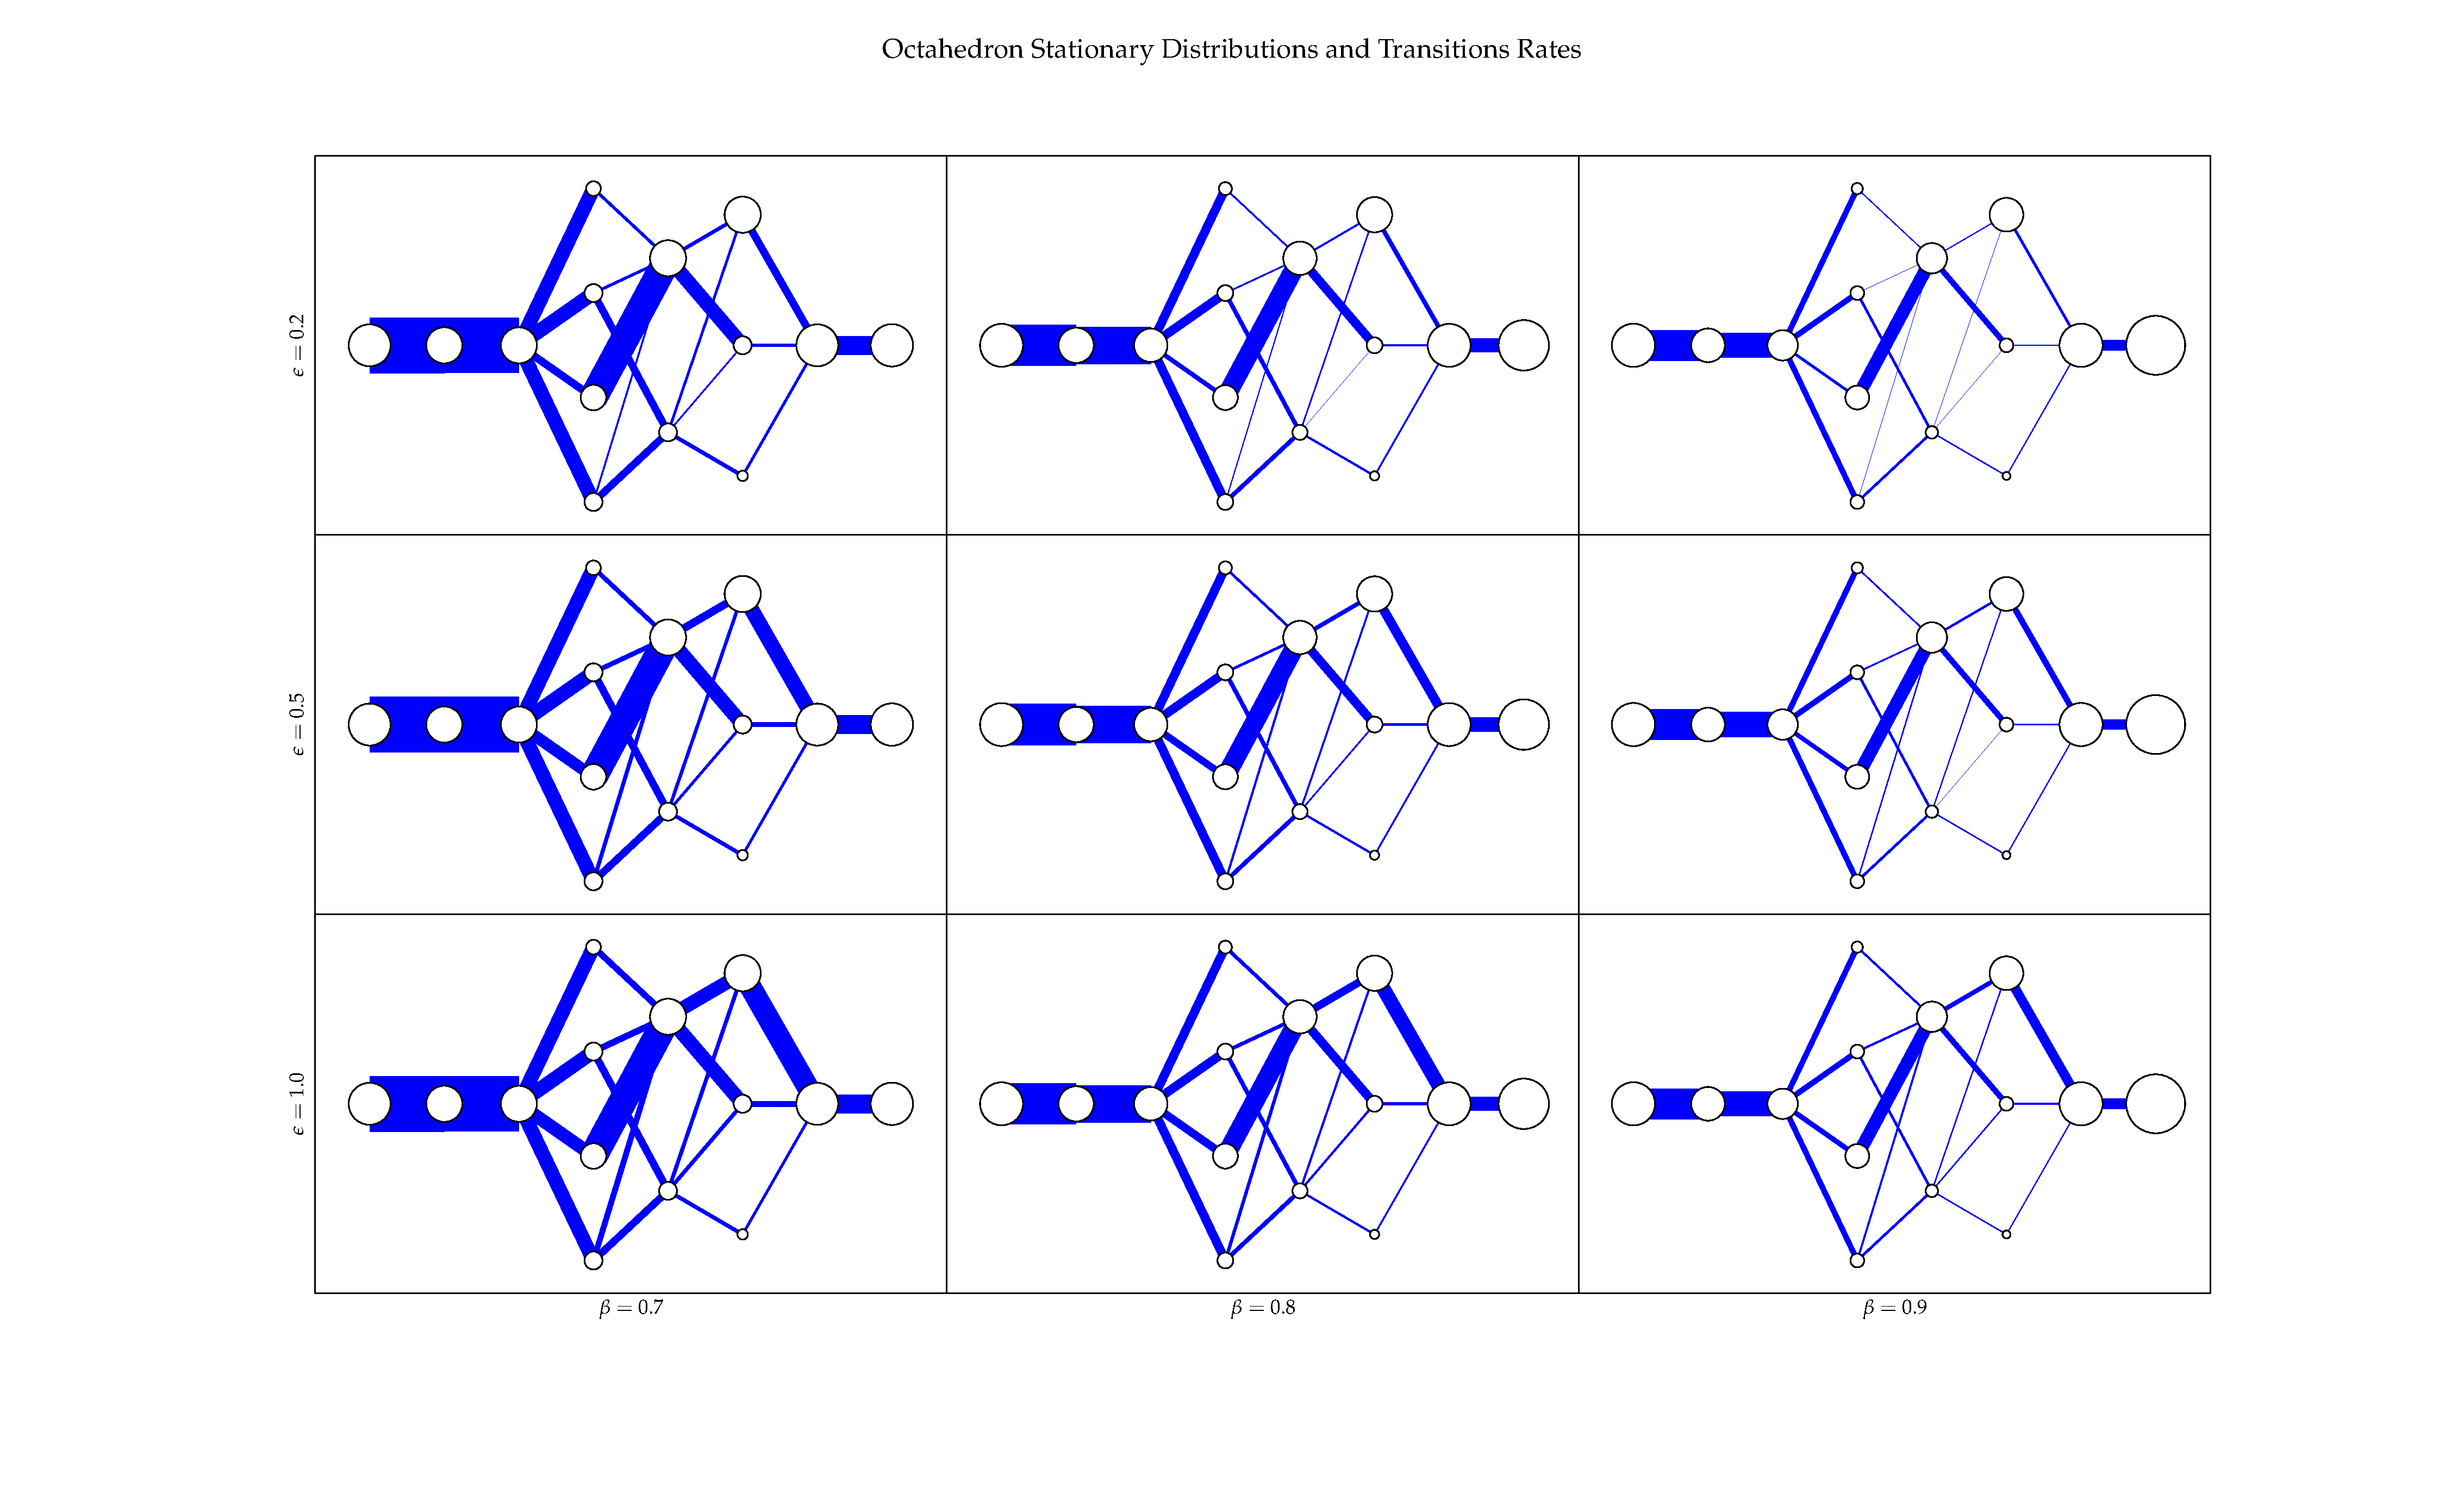
\includegraphics[scale=0.22]{images/octahedron_pi_Q_grid.eps}
\caption{The Affect of $\beta$ and $\epsilon$ on the transitions rates and stationary distribution of the Octahedron combinatorial configuration space.}
\label{fig:OctaPiGrid}
\end{figure}
Figure~\ref{fig:OctaPiGrid} shows how the stationary distributions (node size) and the transition rates (edge thickness) change for three choices of $\epsilon$ and three choices of $\beta$. These plots provide and effective way of visualizing which edges and pathways are more probable for different parameter choices. 

One of the most interesting Markov process statistics is the expected formation time $E[\tau]$.
\begin{figure}[ht]
\centering
  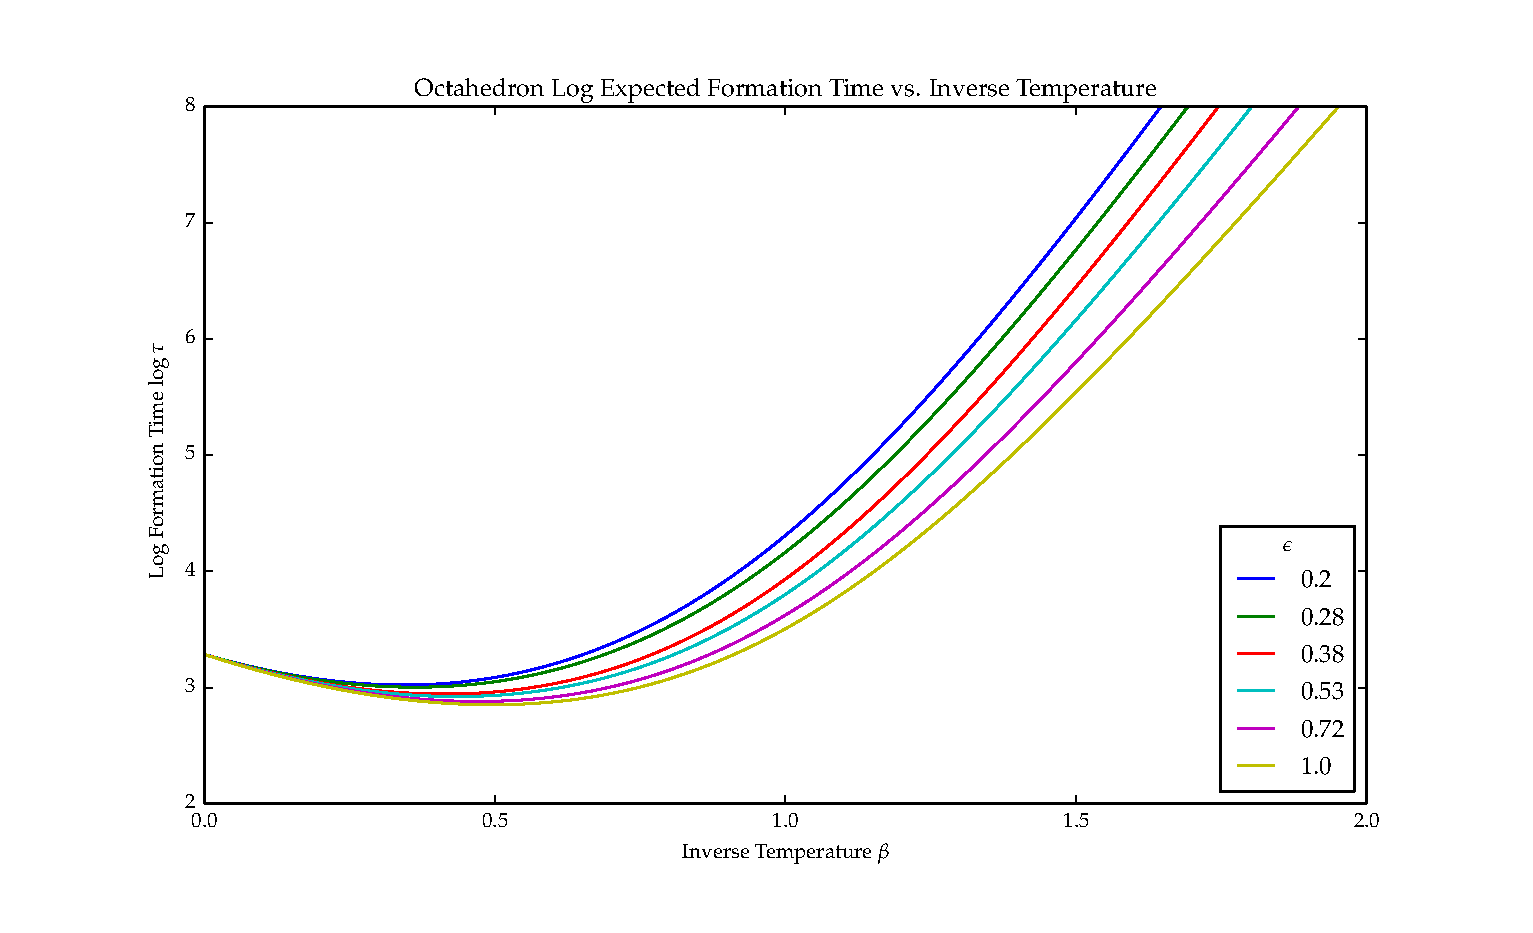
\includegraphics[scale=0.6]{images/octahedron_tau.eps}
\caption{Expected formation times for the octahedron as a function of $\epsilon$ and $\beta$.}
\label{fig:OctaTau}
\end{figure}
Figure~\ref{fig:OctaTau} shows the relation between $\beta$ and the expected formation time for several choices of $\epsilon$. At $\beta = 0$, the Markov process is essentially a random walk on the graph, weighted only by the degeneracy of each transition and unaffected by the choice of $\epsilon$. On the other end, as $\beta$ gets higher and higher, each transition occurs with an increasingly small rate. This leads to a sharp increase in formations times. Interestingly, there is an intermediary range of $beta$s where a minimum of the formation time function occurs. 
